%%%%%%%%%%%%%%%%%%%%%%%%%%%%%%%%%%%%%%%%%%
%Copyright (C) 2018-2019 YuZJ.
%使用CC-BY-NC-SA授权。一份完整版本的许可证已位于附录。这个版本原始作者YuZJ,
%邮箱【邮箱】(最后连接于【时间】)。
%%%%%%%%%%%%%%%%%%%%%%%%%%%%%%%%%%%%%%%%%%
\documentclass{book}
\usepackage{xeCJK} %中文支持
\setCJKsansfont{SourceHanSansCN-ExtraLight.otf}
\setCJKmonofont{SourceCodePro-Light.otf}
\setCJKmainfont{SourceHanSerifSC-ExtraLight.otf}
\setCJKfamilyfont{bolded}{SourceHanSansSC-Bold.otf}
\renewcommand{\bf}{\CJKfamily{bolded}}  
\newcommand{\normalall}{\normalsize\normalfont\normalcolor}  
\usepackage{color}
\usepackage{graphicx}  %生成图片
\usepackage{geometry} %设置页面排版
\geometry{top=0.5in, bottom=0.5in, left=0.5in, right=0.5in, papersize={21cm,29.7cm}}
\usepackage[super]{nth} %生成序数词
\bibliographystyle{unsrt}
\usepackage{metalogo} %生成TeX标志
\usepackage{texnames} %生成TeX标志
\usepackage{fancybox} %生成带阴影的盒子
\shadowsize=2pt %配置盒子
\usepackage{shorttoc}
\usepackage{flafter}%使得所有浮动体不能被放置在其浮动环境之前
\usepackage{picinpar} %生成文本环绕
\usepackage{indentfirst}%生成段落
\usepackage[toc]{multitoc}%双栏目录
\usepackage{amssymb}%显示方块
\makeatletter\renewcommand{\verbatim@font}{\footnotesize \color{blue}\texttt} \makeatletter%修改verbatim环境格式
 %生成章节中文名和盒子
\renewcommand{\thechapter}{\arabic{chapter}}
\renewcommand{\thesection}{\arabic{chapter}.\arabic{section}}
\renewcommand{\thesubsection}{\arabic{chapter}.\arabic{section}.\arabic{subsection}}
\renewcommand{\thesubsubsection}{\arabic{chapter}.\arabic{section}.\arabic{subsection}.\arabic{subsubsection}}
\usepackage{titlesec}
\renewcommand{\bibname}{参考文献}
\renewcommand{\contentsname}{目录}
\renewcommand{\appendixname}{附录}
\titleformat{\chapter}[frame]{\bf \Huge}{\small 第 \thechapter 部分}{0pt}{}
\titleformat{\section}[frame]{\bf  \LARGE}{\small 第 \thesection 章}{0pt}{}
\titleformat{\subsection}[frame]{\bf  \Large}{\small  第\thesubsection 节}{0pt}{}
\titleformat{\subsubsection}[frame]{\bf \large}{\small 第\thesubsubsection 小节}{0pt}{}
\linespread{1.2} %行距命令
\usepackage{eso-pic}%背景图像命令
\usepackage[backref]{hyperref} %生成书签,这个应被放在末尾
\hypersetup{hidelinks,bookmarks=true,bookmarksopen=true,pdftitle=EMACS 26.2中文手册,pdfauthor=YuZJ}
\begin{document}
\setcounter{tocdepth}{5}
\begin{titlepage}	
\AddToShipoutPictureBG*{\includegraphics[width=21cm,height=29.7cm]{pic/face.png}}
{\color{white}{
\vspace*{10mm}
\begin{center}
\doublebox{\parbox{18cm}{
\begin{center}	
\Ovalbox{\Huge \bf EMACS 26.2中文手册\normalsize}\\\vspace*{5mm}\bf \large 作者:YuZJ \\\vspace*{5mm} 编译日期:\today	
\end{center}}}
\end{center}}}
\vspace*{25mm}\normalall
\shadowbox{\parbox[t]{8cm}{{\color{white}{【简介】}}}}
\end{titlepage}
\begin{center}
	\Huge \bf 【版本号】 \normalall
\end{center}
\shorttoc{简明目录}{1}
\tableofcontents
%%%%%%%%%%%%%%%%%%%%%%%%%%%%%%%%%%%%%%%%%%
%Copyright (C) 2018-2020  YuZJLab
%This program is free software: you can redistribute it and/or modify
%it under the terms of the GNU General Public License as published by
%the Free Software Foundation, either version 3 of the License, or
%(at your option) any later version.
%This program is distributed in the hope that it will be useful,
%but WITHOUT ANY WARRANTY; without even the implied warranty of
%MERCHANTABILITY or FITNESS FOR A PARTICULAR PURPOSE.  See the
%GNU General Public License for more details.
%You should have received a copy of the GNU General Public License
%along with this program.  If not, see <https://www.gnu.org/licenses/>.
%%%%%%%%%%%%%%%%%%%%%%%%%%%%%%%%%%%%%%%%%%
\chapter{The Organization of the Screen:屏幕的组织结构}
On a graphical display, such as on GNU/Linux using the X Window System, Emacs occupies
a graphical window. On a text terminal, Emacs occupies the entire terminal screen. We
will use the term frame to mean a graphical window or terminal screen occupied by Emacs.
Emacs behaves very similarly on both kinds of frames. It normally starts out with just one
frame, but you can create additional frames if you wish (see Chapter 18 [Frames]).
\par
在一个图形界面(例如,使用X Windows系统的GNU/Linux操作系统)中,Emacs占用了一个图形窗口(Window)。在一个文本终端中,Emacs占用了一整个终端屏幕。我们将会使用“窗体”(Frame)表示Emacs占用的图形窗体或终端屏幕。Emacs在这两种窗体下表现十分相似\footnote{译注:虽然我不这么认为}。一般情况下Emacs在启动时创建一个窗体,但是你可以按照你的意愿创建另外的窗体(参见第18章【窗体】)。\par
Each frame consists of several distinct regions. At the top of the frame is a menu bar,
which allows you to access commands via a series of menus. On a graphical display, directly
below the menu bar is a tool bar, a row of icons that perform editing commands when you
click on them. At the very bottom of the frame is an echo area, where informative messages
are displayed and where you enter information when Emacs asks for it.
\par
Emacs窗体包括多个区分明显的区域。在窗体的最顶端是菜单栏(Menu Bar),它允许你通过一系列菜单访问命令。在一个图形界面上,菜单栏下方是工具栏(Tool Bar)。它由一系列图标构成,当你单击它是它将执行编辑命令。回显区(Echo Area)窗体的最底端,用于显示Emacs的提示信息或者当Emacs需要你输入时键入信息。\par
The main area of the frame, below the tool bar (if one exists) and above the echo area, is
called the window. Henceforth in this manual, we will use the word “window” in this sense.
Graphical display systems commonly use the word “window” with a different meaning; but,
as stated above, we refer to those graphical windows as “frames”.
\par
在一个Emacs窗体中,位于工具栏(如果存在的话)以及回显区的大块区域称为窗格(Window)。此后我们将会使用“窗格”来表示这个意思。图形界面系统一般会使用“窗口”(Window)来表示不同的意思;但是,正如已经声明的一样,我们将称这些图形界面窗口为“窗体”(Frame)。\par
An Emacs window is where the buffer—the text or other graphics you are editing or
viewing—is displayed. On a graphical display, the window possesses a scroll bar on one
side, which can be used to scroll through the buffer. The last line of the window is a mode
line. This displays various information about what is going on in the buffer, such as whether
there are unsaved changes, the editing modes that are in use, the current line number, and
so forth.
\par
缓冲区(Buffer)——文本、图像以及其他你正在编辑或浏览的东西所显示的地方——位于Emacs窗口。在一个图形界面上,窗格\footnote{译注:是“Window”。此后窗格一律称“Window”,窗体一律称“Frame”。窗口?那是什么东西?}拥有一个纵向的滚动条用于滚动显示整个缓冲区。窗格的最底端一栏(在终端界面下是一行文字)称为状态栏(Mode Line),用于显示关于缓冲区中正在进行的操作的的信息,比如说是否有未保存的改变,正在使用的编辑模式(Editing Mode),当前的行号等等。\par
When you start Emacs, there is normally only one window in the frame. However, you
can subdivide this window horizontally or vertically to create multiple windows, each of
which can independently display a buffer (see Chapter 17 [Windows]).
\par
通常情况下,当你启动Emacs的时候,一个窗体中只有一个窗格。但是,你可以将这个窗格水平或竖直地分为多个窗格,它们各自独立地显示一个缓冲区(参见第17章【窗格】)。\par
At any time, one window is the selected window. On a graphical display, the selected
window shows a more prominent cursor (usually solid and blinking); other windows show a
less prominent cursor (usually a hollow box). On a text terminal, there is only one cursor,
which is shown in the selected window. The buffer displayed in the selected window is
called the current buffer, and it is where editing happens. Most Emacs commands implicitly
apply to the current buffer; the text displayed in unselected windows is mostly visible for
reference. If you use multiple frames on a graphical display, selecting a particular frame
selects a window in that frame.\par
在任何时候,有且仅有一个窗格是活动窗格(Selected Window)。在一个图形界面下,活动窗格显示一个更加明显的光标(Crusor)(一般是闪动的黑色方块“$\blacksquare$”);其它窗格显示一个不明显的光标(一般是空心方块“$\square$”)。终端界面只将在活动窗格显示一个光标。在活动窗格显示的缓冲区称为活动缓冲区(“Selected Buffer”)并且就是正在被编辑的缓冲区。大部分Emacs命令含蓄地作用于活动缓冲区;在非活动的缓冲区中显示的文字仅仅为参考而显示。如果你使用多窗体的图形界面,选择一个窗体再选择一个窗格。
\begin{center}
	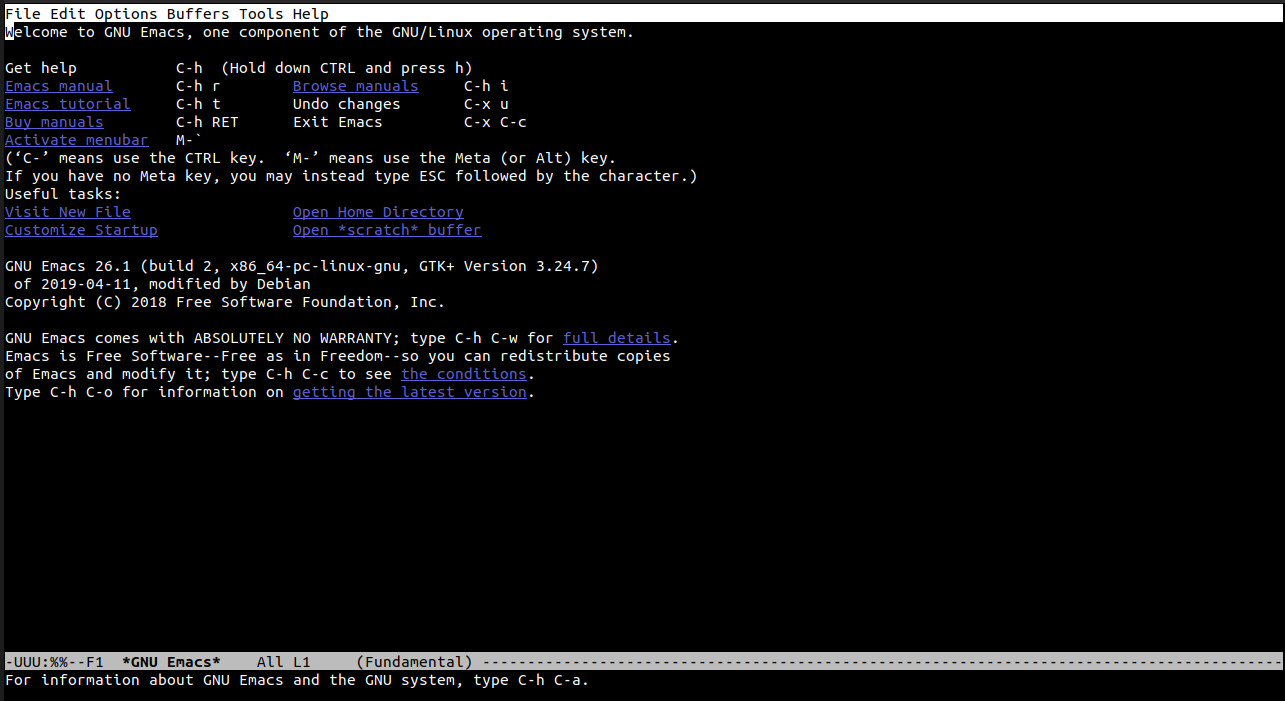
\includegraphics[scale=0.4]{pic/Emacs-Terminal-Defaut}
\end{center}
\section{Point:点}
The cursor in the selected window shows the location where most editing commands take effect, which is called point\footnote{The term “point” comes from the character ‘.’, which was the command in TECO (the language in which the original Emacs was written) for accessing the editing position.}. Many Emacs commands move point to different places in the buffer; for example, you can place point by clicking mouse button 1 (normally the left button) at the desired location.\par
位于被选中窗口的光标(称作“点”,point\footnote{“点”来自于字符“.”,是TECO语言(最初的Emacs由该语言写成)用于连接到正在编辑的位置的命令。})显示了大多数编辑命令生效的位置。许多Emacs的命令能够在缓冲区之内移动光标
\appendix
\renewcommand{\thechapter}{\arabic{chapter}}
%%%%%%%%%%%%%%%%%%%%%%%%%%%%%%%%%%%%%%%%%%
%Copyright (C) 2018-2019 【作者】.
%使用CC-BY-NC-SA授权。一份完整版本的许可证已位于附录。这个版本原始作者【作者】,
%邮箱【邮箱】(最后连接于【时间】)。
%%%%%%%%%%%%%%%%%%%%%%%%%%%%%%%%%%%%%%%%%%
\chapter{附录}
\section{跋}
【跋】
\section{关于本书}
在这里你能读到一些关于本书的信息。
\subsection{版本历史}
开始编写:【时间】\par
编译日期:\today \par
使用\XeLaTeX 编译,\BIBTEX 管理文献。
【版本号】
\subsection{我该如何对这个工程做出贡献?}
请将更改的内容或需要反馈的错误写成一个txt文件,它应该像这样子:
\begin{verbatim}
【工程名称】:【工程网络地址】
[版本号]
[错误性质]
[详细内容]
##解释:
##[版本号]应为所使用的提交的哈希值(如【哈希值】)。
##[错误性质] 应为以下内容中的任意一个:
##[REF]引用错误;侵权
##此时[详细内容]就应该包括具体的内容,在整个PDF文件中的位置,正确的来源
##以及是否可以在修正后继续使用。
##[CONT]内容错误
##此时[详细内容]就应该包括具体的内容,在整个PDF文件中的位置,正确的内容。
##[COMP]编译错误
##此时[详细内容]可省略。
\end{verbatim} \par
例如:
\begin{verbatim}
【工程名称】:【工程网络地址】
[CONT]
commit 【哈希值】
内容略。
\end{verbatim} \par
目前【作者】管理能力有限,因此请不要fork此项目或直接推送更改。
\subsection{感谢}
【感想】
\subsection{商标确认}
所有商标的所有权归各自的商标所有者。
\subsection{编译方法}
对于Windows操作系统,请按以下步骤操作:\par
1.确保您的计算机操作系统为Windows7 sp1及以上。安装TeXLive或2019,并确保“C:/texlive/2019/bin/Win32/ ”目录(这是默认安装路径)已被添加到PATH环境变量中,安装并更新所有宏包。\par
2.运行Compile.bat(在一般的Windows系统下双击即可),它应位于源码包的根目录内。\par
3.如果您希望手动编译,请在根目录内打开命令提示符,按顺序输入如下命令:
\begin{verbatim*}
xelatex Main
bibtex Main
xelatex Main
xelatex Main
del *.log
del *.aux
del *.bbl
del *.blg
del *.toc
del *.out
del *.fls
del *.fdb_latexmk
del *.syntex.gz
\end{verbatim*}
对于GNU/Linux操作系统,请按以下步骤操作:\par
1.安装TeXLive 2019,并确保“/usr/local/texlive/2019/bin/x86\_64-linux/ ”目录(这是默认安装路径)已被添加到PATH环境变量中,安装且更新所有宏包。\par
2.运行Compile.sh(在目录内打开(伪)终端,输入“./Compile.sh”。可能需要先运行“chmod +x Complie.sh”),它应位于源码包的TeX目录内。\par
3.如果您希望手动编译,请在TeX目录内打开(伪)终端,按顺序输入如下命令:
\begin{verbatim*}
xelatex Main.TeX
bibtex Main
xelatex Main.TeX
xelatex Main.TeX
rm -f *.log
rm -f *.aux
rm -f *.bbl
rm -f *.blg
rm -f *.toc
rm -f *.out
rm -f *.fls
rm -f *.fdb_latexmk
\end{verbatim*}
无论你使用何种编译方式,你最终将会得到Main.PDF。这就是最终的文件。
\subsection{关于作者}
【关于作者】
\section{署名-非商业性使用-相同方式共享 3.0中国大陆}
本作品(定义如下)的提供是以适用“知识共享公共许可协议”( 简称“CCPL”或 “许可”)\footnote{来源:【知识共享许可协议法律文本】\url{https://creativecommons.org/licenses/by-nc-sa/3.0/cn/legalcode}(最后访问于2019年6月23日10:47:30)}为前提的。本作品受《中华人民共和国著作权法》以及其他可适用法律的保护。对本作品的使用不得超越本许可协议授权的范围。\par
如您行使本许可授予的使用本作品的权利,就表明您接受并同意遵守本许可协议的所有条款。鉴于本许可为合同,在您接受这些条款和规定的前提下,许可人授予您本许可所包括的权利。
\subsection{第一条\ 定义} 
\begin{enumerate}
	\item 本作品:指根据本许可协议提供的以任何方式和形式(包括以数字形式)表达之文学、艺术和科学领域的作品,例如:书籍、手册等文字作品;讲课、演讲、讲道及其他同类性质的作品;戏剧或音乐戏剧作品;曲艺作品;舞蹈作品及哑剧作品;配词或不配词的音乐作品;电影作品和以类似摄制电影的方法创作的作品;素描、绘画、书法、建筑、雕塑、雕刻或版画等作品;摄影作品以及以类似摄影的方法创作的作品;杂技艺术作品;实用艺术作品;与地理、地形、建筑或科学有关的插图、地图、设计图、草图及立体的造型作品;以及法律、行政法规规定的其他文学艺术作品。为本许可协议之目的,本协议有关“本作品”的规定适用于表演、录音制品及广播电视节目。 
	\item 原始作者:就文学或艺术作品而言,指创作本作品的自然人或依法视为本作品作者的法人或其他组织。为本许可之目的,下述情形下的自然人、法人或其他组织适用本许可有关“原始作者”的规定:(1)就表演而言,指演员、歌唱家、音乐家、舞蹈家和其他表演、演唱、演说、朗诵、演奏、表现或者以其它方式表演文学、艺术作品或民间文学艺术的人员;(2)就录音制品而言,指首次将表演的声音或其他声音录制下来的自然人、法人或其他组织;(3)就广播电视节目而言,指传播广播电视节目的组织;(4)作者身份不明的,指行使作品著作权(除署名权外)的作品原件所有人(比如出版社)。
	\item 演绎作品:指基于本作品,或基于本作品与其他已存在的作品而创作的作品,例如翻译、改编、编曲或对文学、艺术和科学作品的其他变更,包括以摄制电影的方法对作品的改编,或其他任何对本作品进行改造、转换、或改编后的形式,包含任何可确认为源自原始作品的修改形式。在本许可定义之下构成汇编作品的作品不视为演绎作品。为避免疑义,并为本许可之目的,当演绎对象为音乐作品时,将其依时间序列关系与动态影像配合一致而形成的结果,视为演绎作品。
	\item 汇编作品:指由于对内容的选择和编排具有独创性而构成智力创作的文学、艺术或科学作品的集合,其中本作品以完整且未经修改的形式和另外一部或多部作品组成集合的整体,而各组成作品本身是分开且独立的,例如百科全书、文选、数据汇编作品,以及本条第1项所列作品之外的作品或者标的。在本许可定义之下构成汇编作品的作品不视为演绎作品(定义如上)。
	\item 许可人:指根据本许可提供本作品的自然人、法人或者其他组织。
	\item 您:指以前就本作品没有违反过本许可协议、或曾违反过协议但已获得许可人明示同意、依据本许可行使权利的自然人、法人或者其他组织。
	\item 授权要素:是指许可人所选择的、并标示在本许可文本标题中的下列基本属性:署名、非商业性使用、相同方式共享。
	\item 发行:指以出售或者其他权利移转方式向公众提供本作品或者演绎作品的原件或者复制件。
	\item 公开传播:指公开朗诵本作品以及以任何方式或程序,包括以有线、无线的方式或通过信息网络公开传播本作品的公开朗诵;或向公众提供本作品,使公众可以在自己选定的地点获得本作品;或以任何方式或程序公开表演本作品或向公众传播本作品的表演,包括通过信息网络传播本作品的表演;或以任何方式,包括符号、声音或图像,广播或转播本作品。上述定义包括相关法律规定的“展览”“表演”“放映”“广播”或通过信息网络向公众传播作品等传播方式。
	\item 复制:指以印刷、复印、拓印、录音、录像、翻录、翻拍等方式制作本作品的复制件。
	\item 人身权:指相关法律赋予作者对本作品所享有的发表权、署名权、修改权以及保护作品完整权。
\end{enumerate}
\subsection{第二条\ 合理使用}
本许可无意削减、限制或约束您基于《中华人民共和国著作权法》或其他相关法律有关著作权保护的限制或例外的规定对本作品的合理使用。
\subsection{第三条\ 授权}
根据本许可的条款和条件,许可人在此授予您全球性、免版税、非独占并且在本作品的著作权存续期间内均有效的许可,就本作品行使以下权利:
\begin{enumerate}
	\item 复制本作品或将本作品收入一个或多个汇编作品中,以及复制汇编作品中收录的本作品;
	\item 创作和复制演绎作品,但是任何演绎作品,包括任何形式的翻译作品,均需以合理方式清楚地标示、区分或以其他方法表明原始作品已经被修改或变更。例如,翻译作品可以标明“原作品已由英文翻译为西班牙文”,改编作品可以标明“原作品已作修改”;
	\item 发行、公开传播本作品(包括汇编作品中收录的本作品); 
	\item 发行、公开传播演绎作品。
\end{enumerate}
以上权利可在任何现有的或者以后出现的并为可适用的法律认可的媒体和形式上行使。上述权利包括为在其他媒体和形式上行使权利而必须进行技术性修改的权利。许可人在此保留所有未明示授予的权利,包括但不限于第四条第5项所规定的权利。
\subsection{第四条\ 限制}
第三条的授权须受以下规定的限制: 
\begin{enumerate}
	\item 您在发行或公开传播本作品时,必须遵守本许可协议。在您发行或公开传播的本作品的每一份复制件中,您必须附上一份本许可协议的复制件或本许可协议的网址(Uniform Resource Identifier)。您不得就本作品提出或增加任何条款,从而限制本许可协议或者限制获得本作品的第三方行使本许可协议所赋予的权利。您不得对本作品进行再许可。您必须在您发行或公开传播的每份作品复制件中完整保留所有与本许可协议及免责条款相关的声明。 在发行或公开传播本作品时,您不得对本作品施加任何技术措施,从而限制从您处获得本作品的第三方行使本许可协议授予的权利。本项(第四条第1项)规定同样适用于收录在汇编作品中的本作品,但并不要求汇编作品中除本作品外的其他作品受本许可协议的约束。在创作汇编作品时,若接到任一许可人的通知,您必须按照其要求,在可行范围内删除汇编作品中根据本协议第四条第4项的要求所作的有关原始作者的身份及其他有关原始作品相关信息的标注。在创作演绎作品时,若接到任一许可人的通知,您必须根据其要求,在可行范围内删除演绎作品中根据第四条第4项的要求所作的有关原始作者的身份及其他有关原始作品的相关信息的标注。
	\item 您必须以下述许可条款发行或公开传播演绎作品:(1)本许可协议;(2)与本许可协议具有相同授权要素的后续版本;或者(3)与本许可协议具有相同授权要素的其他司法管辖区的知识共享许可协议或其后续版本(例如:署名-非商业性使用-相同方式共享 3.0 美国)(以上三类协议统称为“可适用的协议”)。在您发行或公开传播的每件演绎作品的复制件中,您必须附上一份“可适用的协议”的复制件或网址。您不得就演绎作品提出或增加任何条款,从而限制“可适用的协议”的规定,或者限制获得演绎作品的第三方行使“可适用的协议”所赋予的权利。在发行或公开传播包含本作品的演绎作品时,您必须在本作品的每一份复制件中完整地保留所有与“可适用的协议”及免责条款相关的声明。在发行或公开传播演绎作品时,您不得对演绎作品施加任何技术措施,从而限制从您处获得演绎作品的第三方行使“可适用的协议”所赋予的权利。本项(第四条第2项)规定同样适用于收录在汇编作品中的演绎作品,但并不要求汇编作品中除基于本作品而创作的演绎作品之外的其他作品受“可适用的协议”的约束。 
	\item 您不得以任何形式行使本协议第三条授予您的权利去谋取或获得商业利益或私人金钱报酬。若交换过程中未涉及任何商业利益或私人金钱报酬,通过数字文件共享方式或其他方式用本作品去交换其他受著作权保护的作品,将不被视为谋取或获得商业利益或私人金钱报酬。
	\item 在发行或公开传播本作品、任何演绎作品或汇编作品时,除非有依据第四条第1项之要求,否则您必须完整保留所有关于本作品的著作权声明,并以适于所使用的媒介或方法的形式提供下述信息:(1)在原始作者的姓名(或笔名)已被提供的情况下,给出该姓名或笔名,或者在原始作者或许可人以许可人的著作权声明或其他合理的方式,指定可以在作品上署名的他方当事人姓名的情况下,指明该他方当事人的名称(“署名人”);(2)在本作品标题已被提供的情况下,给出本作品的标题;(3)在合理可行的范围内,标明许可人指定需与本作品同时出现的网址,除非该网址没有涉及到本作品的著作权声明或者关于本作品的许可信息;(4)若为演绎作品,则依第三条第2项之要求,必须注明演绎作品中使用的本作品的作者姓名和作品名称(例如,“某作者作品的法语译本”,或“基于某作者作品的电影剧本”)。本项(第四条第4项)要求的对作者姓名和作品名称的指明可采取任何合理方式,但在演绎作品或汇编作品中,如果已经指明了演绎作品的所有作者或汇编作品中所有内含作品的作者,那么对本作品名称和作者姓名的指明须同时出现在任何其他作者姓名出现的地方,并至少与对其他作者的指明一样显著。为避免疑义,本条有关标示作者姓名和作品名称之规定,仅适用于前述署名的用途;除非您事先另行取得原始作者、许可人或署名人的书面同意,否则您不得以明示或者默示的方式主张或暗示,您本人或您对作品的使用与原始作者、许可人或署名人有关联或者已获得上述人士的赞助或者支持。
	\item 为避免疑义,针对不同司法管辖区的著作权许可体系作出如下约定:
	\subitem 权利不能放弃的强制许可体系。在那些许可人不能放弃通过任何法定的或强制的许可方案收取许可使用费的权利的司法管辖区,许可人保留因您行使本许可协议授予的权利而向您收取许可使用费的专有权;
	\subitem 权利可以放弃的强制许可体系。在那些许可人可以放弃通过任何法定的或强制的许可方案收取许可使用费的权利的司法管辖区,许可人放弃因您行使本许可协议授予的权利而向您收取许可使用费的专有权;但若您行使本许可协议授予的权利时未遵守本许可协议第四条第3项有关非商业性使用的规定,则许可人保留向您收取本作品许可使用费的权利;
	\subitem 自愿许可体系。在实行著作权自愿许可的司法管辖区,若您行使本许可协议授予的权利时未遵守本许可协议第四条第3项有关非商业性使用的规定,则许可人保留向您收取本作品许可使用费的权利,许可人可以自行或者通过所参加的著作权集体管理组织向您收取本作品的许可使用费。
	\item 除非其他法律法规另有规定,您在复制、发行或者公开表演本作品,或者复制、发行或者公开表演作为任何演绎作品或汇编作品一部分的本作品时,不得歪曲、损害或者以其他方式损害本作品,导致原始作者的名誉或者荣誉受损。
\end{enumerate}
\subsection{第五条\ 声明、保证和免责}
除非本许可的当事人相互以书面的方式做出相反约定,且在相关法律所允许的最大范围内,否则许可人按其现状提供本作品,对本作品不作任何明示或者默示、依照法律或者其他规定的陈述或担保,包括但是不限于任何有关可否商业性使用、是否符合特定的目的、不具有潜在的或者其他缺陷、准确性或者不存在不论能否被发现的错误的担保。有些司法管辖区不允许排除前述默示保证,因此这些排除性规定并不一定适用于您。
\subsection{第六条\ 责任限制}
除非属于相关法律所要求的范围,许可人在任何情况下都不对您因本许可或因使用本作品而产生的任何直接损失、间接损失或惩罚性赔偿负责,即使许可人已被告知发生此类损害的可能性。 
\subsection{第七条\ 许可终止}
\begin{enumerate}
	\item 在您违反本许可协议任何条款时,本许可及其所授予的权利将自动终止。然而,根据本许可从您处获取演绎作品或汇编作品的自然人、法人或者其他组织,如果他们仍完全遵守相关条款,则对他们的许可不会随之终止。即使本许可被终止,第一条、第二条、第五条、第六条、第七条以及第八条仍然有效。
	\item 在上述条款及条件的前提下,此处授予的许可在法定著作权保护期限内有效。即便如此,许可人保留依其他许可条款发行本作品及在任何时候停止发行本作品的权利;但是,许可人的上述权利不能被用于撤销本许可或任何其他在本许可条款下授予的或必须授予的许可,除本条第1项指明的终止外,本许可将保持其完全效力。
\end{enumerate}
\subsection{第八条\ 其他事项}
\begin{enumerate}
	\item 当您发行、公开传播本作品或其汇编作品时,许可人给获得作品的第三方提供本作品的许可,其条款和条件与您所获得的许可相同。
	\item 当您发行或公开传播演绎作品时,许可人给获得作品的第三方提供本作品的许可,其条款和条件与您所获得的许可相同。
	\item 如因相关法律,本许可的某一条款无效或不能履行,本许可其余条款的有效性和可履行性不受影响。如本许可的当事人未采取进一步措施,此类无效条款应在必要范围内进行最低限度的修改以使其有效和可履行。
	\item 除非当事人书面同意并签字放弃某条款和允许某违约行为,本许可的任何条款或规定都不应被视为已被放弃,或被视为允许此违约行为。
	\item 本许可构成相关当事人与本授权作品相关的全部协议。除已在此处确认的之外,并不存在任何与本作品相关的谅解备忘录、协议或声明。许可人不受您提出的任何附加规定的约束。未经许可人和您双方书面同意,本许可不得更改。
\end{enumerate}
\subsection{“知识共享”(Creative Commons)声明}
“知识共享”不是本许可协议的一方,对本作品不作任何相关保证。“知识共享”不对您或任何其他方的任何损失负责,包括但不限于与本许可相关的直接损失和间接损失。虽然有上述两点,但如果“知识共享”已明确标识自己为许可人,它将承担许可人的全部权利和义务。\par
除用于向公众表明本作品是依照知识共享公共许可协议(CCPL)授权以外,如未经“知识共享”事先书面同意,任何一方均不得使用“知识共享”(Creative Commons)商标和其他相关商标及标识。任何被允许的使用都必须符合“知识共享”的现行商标使用准则。该准则已在其网站上发布或可应要求随时提供。为避免疑义,本段关于商标的限制性规定不构成本许可之一部分。\par
您可以通过\url{https://creativecommons.org/}(最后连接于2019年6月23日10:57:40)联系“知识共享”
\addcontentsline{toc}{chapter}{参考文献}
\bibliography{Reference}
全书结束。
\end{document}
